\newpage
\section{Provas}

\subsection{\textsc{Subset-Sum} está em \textbf{NP}}

Dado que \textbf{NP} é o conjunto dos problemas de decisão em que uma possível solução pode ser verificada em tempo polinomial, para mostrar que \textsc{Subset-Sum} está em \textbf{NP} para uma instância $\langle S, t \rangle$ do problema, toma-se o subconjunto $S'$ para ser verificado. O Algoritmo~\ref{alg:check} de verificação pode checar se $\sum_{s \in S'} s = t$ em tempo polinomial $O(n)$.

\begin{algorithm}[h]
	\KwIn{$\langle S', t \rangle$}
	\KwOut{\textit{true} se $S'$ é solução, \textit{false} caso contrário}

	$sum \leftarrow 0$\;
	\ForEach{$s \in S'$}{
		$sum \leftarrow sum + s$\;
	}
	\If{$sum = t$}{
		\Return{true}\;
	}
	\Return{false}\;
\caption{Verifica uma solução $S'$ do \textsc{Subset-Sum} em tempo polinomial. \label{alg:check}}
\end{algorithm}

\subsection{\textsc{Subset-Sum} é \textbf{NP}-\textit{completo}}

\subsubsection{Redução}

Antes de provar a \textbf{NP}-\textit{completude} do \textsc{Subset-Sum}, é necessário conhecer os problemas canônicos usados para prová-lo por \textbf{redução}.

A técnica de provar por redução que um problema $B$ é \textbf{NP}-\textit{completo}, requer conhecer um problema $A$ que já foi provado ser \textbf{NP}-\textit{completo} e então encontrar uma maneira de reduzir $A \rightarrow B$ ``refraseando'' $A$ ou encontrando um algoritmo que converta qualquer instância de $A$ em uma instância de $B$ em tempo polinomial. Assim, pode-se dizer que $B$ é tão difícil quanto $A$, ou ainda, que $B$ não é mais do que um fator polinomial difícil do que $A$.

Ou seja, se $A \leq_{\textbf{P}} B$ e $A \in$ \textbf{NP}-\textit{completo} $\Rightarrow$ $B \in$ \textbf{NP}-\textit{completo}.

\subsubsection{Problemas de Satisfatibilidade Conhecidos}

\textbf{\textsc{Circuit-Sat}} é um problema canônico de satisfatibilidade provado pertencer a \textbf{NP}-\textit{completo}. Seu enunciado é: dado um circuito booleano combinacional, ele é satisfatível?

Ou, mais formalmente como uma linguagem:
	
\textsc{Circuit-Sat} $ = \{ \langle C \rangle$ : $C$ é um circuito booleano combinacional satisfatível $\}$.

Um circuito booleano combinacional é um conjunto de variáveis que podem receber os valores 0 (\textit{false}) ou 1 (\textit{true}) e que de acordo com as operações lógicas AND ($\land$), OR ($\lor$) e NOT ($\lnot$) pode resultar em uma resposta 0 ou 1. Dado um circuito $C$, pode-se determinar se ele é satisfatível simplesmente testando todas as atribuições possíveis para suas $n$ variáveis, que é um total de $2^n$ atribuições.

O \textsc{Circuit-Sat} foi provado ser \textbf{NP}-\textit{completo}, pois, tratando-o mais abstratamente como uma linguagem $L \subseteq \{0,1\}^*$, satisfaz as seguintes propriedades:
\begin{enumerate}[itemindent=1cm]
	\item $L \in \textbf{NP}$, e 
	\item $L' \leq_{\textbf{P}} L$ para todo $L' \in \mathbf{NP}$.
\end{enumerate}

\textbf{\textsc{SAT}} é um problema de decidir se uma fórmula booleana $\phi$ é satisfatível.

Como linguagem:
\textsc{SAT} $= \{ \langle \phi \rangle$ : $\phi$ é uma fórmula booleana satisfatível $\}.$
	
Um fórmula booleana, além dos operadores $\land$, $\lor$, $\lnot$, contém também $\implies$ (implicação) e $\iff$ (se e somente se). O problema \textsc{Circuit-Sat} pode ser reduzido ao \textsc{SAT} e logo também \textsc{SAT} pertence a \textbf{NP}-\textit{completo}.

\textbf{\textsc{3-CNF-SAT}} é um problema de decidir se uma fórmula booleana $\phi$ em 3-CNF é satisfatível.

Como linguagem:
\textsc{3-CNF-SAT} $= \{ \langle \phi \rangle$ : $\phi$ é uma fórmula booleana 3-CNF satisfatível $\}.$

A 3-CNF -- Forma Normal Conjuntiva com 3 literais -- é uma maneira canônica de expressar uma fórmula booleana como uma conjunção de disjunções em que cada cláusula tem exatamente 3 literais -- um literal é a ocorrência de uma variável ou de sua negação. Por exemplo, a seguinte fórmula é 3-CNF: $(x_1 \lor \lnot x_3 \lor \lnot x_2) \land (x_3 \lor x_2 \lor x_4) \land (\lnot x_1 \lor \lnot x_3 \lor \lnot x_4)$. Seguindo o diagrama da Figura~\ref{fig:sat}, o \textsc{3-CNF-SAT} é provado ser \textbf{NP}-\textit{completo} por redução do \textsc{SAT}.

A prova de \textbf{NP}-\textit{completude} dos problemas citados nesta Seção está fora do escopo deste trabalho, mas seu conhecimento é necessário para ser usado na prova de \textbf{NP}-\textit{completude} do \textsc{Subset-sum}.

\begin{figure}[h]
	\centering
	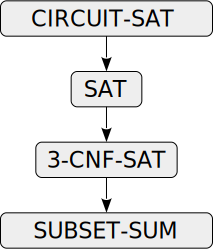
\includegraphics[scale=0.7]{./input/sat.pdf}
	\caption{Dependência de problemas para a prova de \textbf{NP}-\textit{completude} do \textsc{Subset-Sum}. \label{fig:sat}}
\end{figure}

\subsubsection{\textsc{Subset-Sum} usando \textsc{3-CNF-SAT}}

Dada uma fórmula $\phi$ sobre as variáveis $x_1, x_2, \dots, x_n$ com cláusulas $C_1, C_2, \dots, C_k$ cada uma contendo exatamente três literais distintos, o algoritmo de redução contrói uma instância $\langle S, t \rangle$ do \textsc{Subset-sum} tal que $\phi$ é satisfatível se, e somente se, existe um subconjunto de $S$ cuja soma é exatamente $t$.

Toma-se os devidos cuidados para que $\phi$ não contenha um literal e sua negação em uma mesma cláusula e cada variável de $\phi$ apareça pelo menos uma vez em alguma cláusula.

A redução cria dois números em $S$ para cada variável $x_i$ e dois números em $S$ para cada cláusula $C_j$. Assim construímos $S$ e $t$ da seguinte maneira. Para cada valor $s \in S$, nomeamos cada posição de seus dígitos ou por uma variável ou por uma cláusula de $\phi$. Os $k$ menos significantes dígitos de cada $s$ são nomeados pelas cláusulas e seus $n$ mais significantes dígitos são nomeados pelas variáveis.
	
\begin{itemize}
	\item O valor $t$ tem 1 em cada dígito nomeado por uma variável e 4 em cada dígito nomeado por uma cláusula.
	
	\item Para cada variável $x_i$, o conjunto $S$ contém dois inteiros $v_i$ e $v'_i$. Cada $v_i$ e $v'_i$ tem 1 no dígito nomeado por $x_i$ e 0 nos demais dígitos de variáveis. Se o literal $x_i$ aparece numa cláusula $C_j$, então o dígito nomeado por $C_j$ em $v_i$ contém 1. Se o literal $\lnot x_i$ aparece numa cláusula $C_j$, então o dígito nomeado por $C_j$ em $v'_i$ contém 1. Todos demais dígitos nomeados por cláusula em $v_i$ e $v'_i$ são 0.\\
	Dessa maneira, tomado os devidos cuidados citados acima para a fórmula $\phi$, todos os $v_i$ e $v'_i$ são únicos.
	
	\item Para cada cláusula $C_j$, o conjunto $S$ contém dois inteiros $r_j$ e $r'_j$. Cada $r_j$ e $r'_j$ tem 0 em todos os dígitos que não sejam  aqueles nomeados por $C_j$. Para $r_j$, existe um 1 no dígito de $C_j$ e $r'_j$ tem um 2 neste dígito. Esses inteiros são usados para fazer somar até 4 nos dígitos nomeados por cláusulas.
\end{itemize}

Essa redução pode ser feita em tempo polinomial. O conjunto $S$ contruído contém $2n + 2k$ valores $s$, cada um contendo $n + k$ dígitos, e o tempo para produzir cada dígito é $O(n + k)$. O valor $t$ também tem $n + k$ dígitos e também é produzido em tempo polinomial.

Mostra-se agora que a fórmula $\phi$ é satisfatível se, e somente se, existe um $S' \subseteq S$ para os $S$ e $t$ construídos. Primeiro, suponha que existe uma atribuição que satisfaça $\phi$. Para cada $i = 1, 2, \dots, n$, se $x_i = 1$ nessa atribuição, então inclui-se $v_i$ em $S'$. Caso contrário, inclui-se $v'_i$. Dessa maneira, a soma de todos os valores incluídos em $S'$ até agora satisfazem os primeiros $n$ dígitos de $t$. E, para atingir os dígitos 4 de $t$, inclui-se os subconjuntos não-vazios apropriados de variáveis $\{r_j, r'_j\}$ de acordo com as claúsulas $C_j$.

Agora, suponha que existe um subconjunto $S' \subseteq S$ que seus valores some $t$. O subconjunto $S'$ tem que incluir exatamente um $v_i$ ou um $v'_i$ para cada $i = 1, 2, \dots, n$. Caso contrário, os $n$ primeiros dígitos de $t$ não seriam alcançados na soma. E pode-se afirmar que todas claúsulas $C_j$, $j = 1, 2, \dots, n$ também são satisfeitas, pois para alcançar a soma 4 nos $k$ dígitos menos significativos de $t$, o subconjunto $S'$ deve incluir pelo menos um $v_i$ ou um $v'_i$ que tem dígito 1 em $C_j$, e uma vez que as contribuições $r_j$ e $r'_j$ somam no máximo 3, consegue-se totalizar os valores 4 para esses $k$ dígitos.

\newpage
Por exemplo: para $\phi = C_1 \land C_2 \land C_3 \land C_4$, onde $C_1 = (x_1 \lor \lnot x_2 \lor \lnot x_3)$, $C_2 = (\lnot x_1 \lor \lnot x_2 \lor \lnot x_3)$, $C_3 = (\lnot x_1 \lor \lnot x_2 \lor x_3)$ e $C_4 = (x_1 \lor x_2 \lor x_3)$, uma atribuição que satisfaz $\phi$ é $\langle x_1 = 0, x_2 = 0, x_3 = 1 \rangle$. O conjunto $S$ construído pela redução é $S$ = \{ 1001001, 1000110, 100001, 101110, 10011, 11100, 1000, 2000, 100, 200, 10, 20, 1, 2 \} e $t = 1114444$. Como ilustrado na Figura~\ref{fig:reducao}.

\begin{figure}[h]
	\centering
	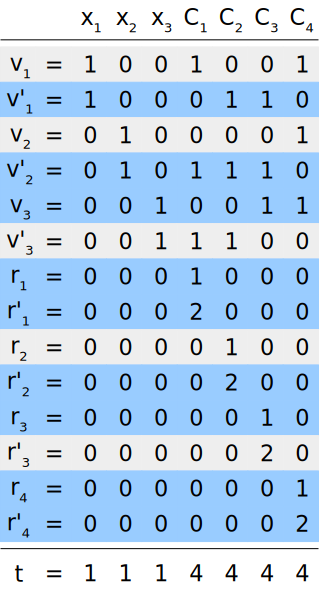
\includegraphics[scale=0.70]{./input/reducao.pdf}
	\caption{Ilustração do conjunto $S$ para uma fórmula $\phi$. As linhas em azul claro são os valores de $S'$ que satisfazem a soma $t$. \label{fig:reducao}}
\end{figure}

